\section{Cinemática} \label{sec:cinematica}

La cinematica es una parte de la fisica que estudia el movimiento de los sistemas mecanicos sin tomar en cuenta las fuerzas que originan dicho movimiento. Se centra en la relacion geometrica entre las articulaciones del robot y su extremo efector, de esta forma permite predecir la posicion y orientacion en funcion de las posiciones articulares, y viceversa. Comprender la cinematica es vital para entender el comportamiento del robot, hacer el control y diseño del mismo. 

\subsection{Cinemática Directa}
En la cinemática robótica, la cinemática directa consiste en aplicar las ecuaciones del sistema para determinar la ubicación del efector final a partir de valores concretos de las articulaciones.Estas ecuaciones se emplean tanto en robótica como en áreas como los videojuegos y la animación digital. El procedimiento contrario, que busca los valores articulares necesarios para alcanzar una posición deseada del efector, se denomina cinemática inversa.
Las ecuaciones cinemáticas para la cadena en serie de un robot se obtienen utilizando una transformación rígida [Z] para caracterizar el movimiento relativo permitido en cada articulación y una transformación rígida separada [X] para definir las dimensiones de cada eslabón. El resultado es una secuencia de transformaciones rígidas que alternan transformaciones de articulaciones y eslabones desde la base de la cadena hasta su eslabón final, que se equipara a la posición especificada para el eslabón final.

En 1955, Jacques Denavit y Richard Hartenberg propusieron una convención para definir las matrices de unión [Z] y las matrices de enlace [X], con el objetivo de unificar la forma en que se establecen los marcos de coordenadas en sistemas de eslabones espaciales. Esta metodología ubica el marco de referencia de cada unión de manera que su transformación corresponda a un desplazamiento helicoidal (tipo tornillo) a lo largo del eje Z.
El método conocido como Denavit-Hartenberg (DH) se ha convertido prácticamente en un estándar en robótica, ya que permite su implementación automatizada sobre modelos tridimensionales de brazos robóticos.

Un brazo manipulador está compuesto por varios eslabones unidos mediante articulaciones, las cuales pueden ser de tipo rotacional o prismático. Estas articulaciones, al girar o desplazarse linealmente, aportan los grados de libertad necesarios para el movimiento del sistema. Si se conoce la longitud de cada eslabón rígido, la ubicación del efector final puede determinarse completamente a partir de los ángulos articulares y los desplazamientos lineales (en el caso de juntas prismáticas).

Para aplicar correctamente la convención DH, es necesario establecer un sistema de coordenadas en cada articulación. En este marco, el eje z se asigna como el eje de rotación en juntas rotacionales, y como el eje de traslación en juntas prismáticas.

\begin{figure}[H]
    \centering
    
\includegraphics[width=0.85\textwidth]{matriz.png}
    \caption{DH}
    \label{fig:matriz}
\end{figure}

\subsection{Cinemática Diferencial}
El modelo cinemático diferencial (MCD) busca entre otras cosas encontrar la relación existente entre las velocidades articulares y la velocidad del extremo operativo del robot, y por extensión de cualquier otro punto asociado al mismo.
Esta relación, que puede derivarse del modelo cinemático directo previamente estudiado, proporciona información particularmente valiosa. Gracias a ella, es posible identificar las singularidades del sistema, analizar la capacidad de manipulación del robot en el espacio, y sentar las bases para aplicar métodos numéricos que permitan resolver de forma iterativa la cinemática inversa, e incluso controlar el movimiento del robot dentro del espacio de trabajo.

En secciones previas se desarrolló la solución del modelo cinemático directo, el cual permite determinar la posición del efector final en función de las coordenadas articulares q esta relación se expresa como f(q). Utilizando el método de Denavit-Hartenberg y el uso de matrices homogéneas, dicha solución se representa mediante una matriz homogénea resultante del producto sucesivo de matrices

La matriz jacobiana aunque en matemáticas, el concepto de Jacobiana asociado a una función vectorial es claro y unívoco, en robótica se habla de matriz jacobiana siempre que se trate de una matriz que transforma de un sistema de velocidades a otro. Por defecto, cuando se habla de la matriz jacobiana 3de un robot, hablaremos de aquella que relaciona las velocidades articulares con la velocidad espacial, sin embargo existen más jacobianas. Comenzaremos en primer lugar por ver la más sencilla de todas, que es aquella matriz que nos permite transformar un vector de velocidades dado en un sistema de referencia a otro sistema de referencia.

En resumen la cinemática diferencial, dentro del modelo cinemático, tiene como propósito establecer la relación entre las velocidades del punto que se desea controlar, representado como h(x,y), y las velocidades articulares que determinan el movimiento del robot. En este enfoque, se considera al robot como una masa puntual, por lo que no se toman en cuenta las fuerzas involucradas, como los efectos de la inercia o el rozamiento.

\begin{figure}[H]
    \centering
    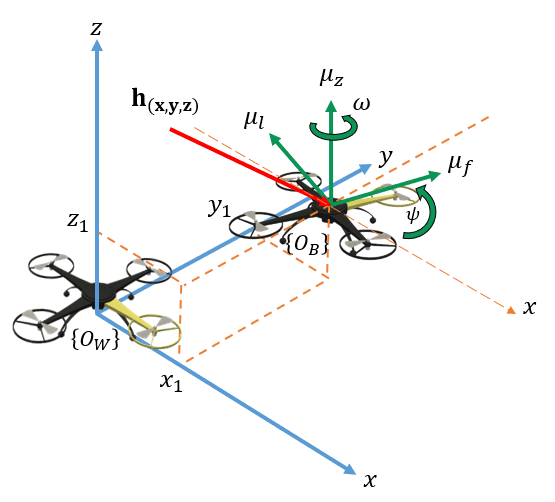
\includegraphics[width=0.50\textwidth]{img/Modelo-cinematico.png}
    \caption{Modelo diferencial}
    \label{fig:Modelo-cinematico}
\end{figure}

\subsection{Cinemática Inversa}
En el ámbito de la robótica, la cinemática inversa se encarga de calcular los valores que deben adoptar las articulaciones para alcanzar una posición y orientación específica del efector final. Esta herramienta es fundamental, ya que aunque el robot realiza sus tareas a través de los efectores, el control real se aplica sobre las articulaciones.
Cuando se desea que el robot pase de una postura inicial a una final determinada, hablamos de planificación de movimiento. La cinemática inversa se utiliza para traducir ese plan en trayectorias que deben seguir los actuadores.

Este mismo principio se aplica en otras áreas, como la animación de personajes en películas, donde es necesario mover las articulaciones para lograr que un personaje adopte ciertas posturas. También se usa en la simulación de vehículos que transportan cámaras —como coches o barcos—, permitiendo calcular cómo cambiaría la perspectiva de la cámara al avanzar, sin que los objetos en el entorno parezcan moverse de manera poco realista.

En general, el movimiento de cualquier cadena cinemática, ya sea un brazo robótico o un esqueleto animado, se modela mediante ecuaciones cinemáticas que describen su configuración a partir de los parámetros articulares. Mientras la cinemática directa determina la posición final a partir de los valores de las articulaciones, la cinemática inversa hace el proceso contrario: encuentra qué valores articulares se necesitan para alcanzar una posición deseada.

